\Chapter{ADAPTIVE SAFE SCREENING METHOD FOR LASSO PENALIZED COX REGRESSION}
\label{METHOD2}

\section{Introduction}

Cox proportional hazards regression \citep{cox1972regression} is a popular method for survival analysis, in which the response is the time to an event, typically a failure time. The main idea of Cox regression is that the predictors have a multiplicative effect on the hazard function. Meanwhile, the shape of the baseline hazard function is left unspecified and assumed to be the same for every subject. Estimation is based on a partial likelihood that considers only the ranks of the failure times, thereby producing a semiparametric method in which the effect of features on relative risk is modeled without assuming a distribution for the failure times. As a result Cox regression is more flexible and robust than parametric survival models, an appealing property since the distribution of failure times is often too complicated for simple parametric models. Cox regression is widely used in many domains including biostatistics, economics, and social science.

However, when the number of features is large, Cox regression, like other regression methods, is prone to over-fitting. Moreover, when the number of features is greater then number of events, the maximum likelihood estimates are no longer unique. Finally, coefficients go to infinity in the case of complete or quasi-complete separation, an event that is increasingly likely to occur as the number of features increase. Regularization methods such as the lasso are effective at dealing with all of these problems \citep{tibshirani1997lasso}. Lasso penalized Cox regression is not only more stable, but carries out automatic feature selection by setting many coefficients equal to zero, and is thus particularly attractive when dealing with high dimensional data. Typical practice is to solve the regression models over a path of decreasing values of the regularization parameter. Efficient algorithms for obtaining the solution path to lasso penalized Cox regression have been previously developed \citep{simon2011regularization}.

In recent years, big data has become more easily accessible and there is an increasing need to study ultra high dimensional data with millions of features. This introduces considerable challenges to existing optimization methods. One promising technique to tackle this challenge is ``screening'', in which ``inactive'' features -- features whose coefficients are equal to zero -- are identified prior to fitting and ``eliminated''. The eliminated features can then be ignored during the optimization, which results in dimension reduction and improvements in computation time and memory cost. The ``strong'' screening rule \citep{Tibshirani2012} was derived in a general form for a class of lasso type problems and the specific applications to lasso penalized Cox regression are also studies \citep{simon2011regularization,yang2013}. It eliminates a large proportion of features but requires a check afterwards to verify that no features were incorrectly eliminated. Another type of screening is ``safe'' rules, which are mathematically guaranteed not to make a mistake and therefore don't require a check. Skipping the post-convergence checking stage saves time in general; however, safe rules are typically less powerful than strong rules in the sense of eliminating fewer features, and which of the two approaches is best in practice depends on a number of factors, as investigated in \citep{Zeng2021}. For lasso penalized Cox regression, the only safe rule that we are aware of is SAFE \citep{ko2017solving}. However, this work is unpublished and there is a mistake in its derivation which makes it unsafe in the presence of tied failure times. Meanwhile, when there are no tied failure times, the SAFE rule is rather weak and eliminates only a small portion of features (if any).

A more powerful class of safe rules takes advantage of the path structure of the solution by utilizing solutions at previous penalty parameter values, thereby greatly increasing the number of features which can be eliminated. Sequential screening can be carried out with such safe rules by always utilizing the previous solution in the path. Moreover, adaptive screening approaches proposed in Chapter \ref{METHOD1} can also use such safe rules: a previous solution can be safely reused multiple times to greatly reduce the computation cost of screening at minimal cost in terms of screening power. Safe rules that utilize previous solutions are both mathematically and computationally more complicated and previous studies have focused almost exclusively on linear regression \citep{wang2013lasso}. A rare exception is the SLORES rule for lasso penalized logistic regression \citep{wang2014safe}, which was first proposed in a manner that does not consider previous solutions but can be extended to utilize previous solutions. This suggests the possibility of extending sequential safe rules to other types of lasso problems and incorporating them into an adaptive screening framework.

In this paper, we develop a novel safe rule for lasso penalized Cox regression that uses previous solutions to improve power. It is based on the dual form of the Cox partial likelihood; by deriving a bound for the dual solution, the rule can identify solutions whose primal coefficients will equal zero without actually solving the primal problem. The power of the proposed rule depends on the tightness of this bound and we discuss conditions under which the screening method is most and least powerful. Finally, we carry out numerical studies to show the advantages and disadvantages of the proposed rule.

\section{Screening Method}
\subsection{Problem Definition}

In a survival analysis, we collect data on $n$ subjects of the form $\{(t_i,y_i,\tilde{x}_i)\}_{i=1}^n$, where $t_i$ is the observed time on study and represents the time of failure if $y_i=1$ or the time of right censoring if $y_i=0$ (i.e., the failure happens at some unknown time after $t_i$), and $\tilde{x}_i=(X_{i1},X_{i2},...,X_{ip})$ is a vector of $p$ features. With these observed data, we can define the following quantities. Let $X=[\tilde{x}_1,\tilde{x}_2,...,\tilde{x}_n]^T=[x_1,x_2,...,x_p]$ denote the $n\times p$ feature matrix. Suppose there are $f$ unique times when at least one failure happens. Let  $\Delta=[\Delta_1,\Delta_2,...,\Delta_f]^T=\{\delta_{ki}\}\in\{0,1\}^{f\times n}$ denote the at-risk matrix, where $\delta_{ki}=1$ if subject $i$ is at risk at the $k$-th unique failure time. Let $Y$ denote the $f\times n$ response matrix where $Y_{ki}=1$ if subject $i$ died at the $k$-th unique failure time and $Y_{ki}=0$ otherwise. Finally, letting $y$ denote the $n \times 1$ response vector of elements $y_i$ and $d$ the $n \times 1$ vector of elements $d_k>0$, where $d_k$ denotes the number of failures at unique failure time $k$, we have $y=Y^T\mathbf{1}$ and $d=Y\mathbf{1}$.

The lasso penalized Cox regression, with the Breslow approximation \citep{breslow1974covariance} for tied failure times, consists of the optimization problem
\begin{equation}
    \label{eq:cox}
    \underset{\beta\in \mathbb{R}^p}{\mathrm{min}}-y^TX\beta+\sum_{k=1}^f d_k\log\left(\sum_{i=1}^n \delta_{ki} e^{\tilde{x}_i^T\beta}\right)+n\lambda||\beta||_1,
\end{equation}
where $\beta\in\mathbb{R}^p$ is the coefficient vector corresponding to the $p$ features and $\lambda>0$ is the regularization parameter that controls the size of lasso penalty. A dual form of \eqref{eq:cox} is given by (see Appendix~\ref{sec:dualcox} for details):
\begin{gather}
        \label{eq:dualTheta}
        \underset{\Theta\in \mathbb{R}^{f\times n}}{\mathrm{min}}g(\Theta)\equiv\sum_{k=1}^f\sum_{i=1}^n\delta_{ki}(Y_{ki}+d_k^{1/2}\Theta_{ki})\log\left(\frac{Y_{ki}}{d_k}+\frac{\Theta_{ki}}{d_k^{1/2}}\right)\\
        \begin{aligned}s.t.\quad \Theta\in \mathcal{F}_\lambda\equiv\{\Theta:\quad
            &||X^T\Theta^Td^{1/2}||_\infty\leq n\lambda,\quad D^{1/2}\Theta+Y+(1-\Delta)> 0,\\& \Theta\circ(1-\Delta)=0,\quad \Theta\mathbf{1}=0\}\nonumber,
        \end{aligned}
\end{gather}
where $\Theta\in \mathbb{R}^{f\times n}$ is the dual variable, $D=\textrm{diag}(d)$, ``$>$'' is element wise greater-than, $(\cdot)^{1/2}$ is the element wise square root, $\circ$ is element wise product, and we define $0\log 0$ to be 0. The dual problem therefore consists of minimizing the convex function $g(\Theta)$ within a convex feasible set $\mathcal{F}_\lambda$. Letting $\beta_\lambda$ denote the solution to the primal problem at penalty parameter value $\lambda$ and $\Theta_{\lambda}$ denote the corresponding dual solution, the primal solution and dual solution are connected by
\begin{equation}
    \label{eq:dualprimalcox}
    [\Theta_\lambda]_{ki}=d_k^{1/2}\delta_{ki}\frac{e^{\tilde{x}_i\beta_\lambda}}{\sum_{i'=1}^n\delta_{ki'}e^{\tilde{x}_{i'}\beta_\lambda}}-d_k^{-1/2}Y_{ki},
\end{equation}
for all $k$ and $i$. Furthermore, the KKT conditions for the primal problem~\eqref{eq:cox} can be expressed as:
\begin{gather}
    \label{eq:kktcox}
    \begin{aligned}&[\beta_\lambda]_{j}=0\implies\left|x_j^T\Theta_\lambda^Td^{1/2}\right|\leq n\lambda\\
    & [\beta_\lambda]_{j}\neq0\implies x_j^T\Theta_\lambda^Td^{1/2}= n\lambda\textit{sign}([\beta_\lambda]_{j}).
    \end{aligned}
\end{gather}
for any $j$. Combining \eqref{eq:dualprimalcox} and \eqref{eq:kktcox}, we can obtain a closed form solution for the problem at large $\lambda$ values:
\begin{gather}
    \label{eq:lammaxcox}
    \begin{aligned}
        \beta_\lambda=0\iff \lambda \geq \lambda_{\max}&\equiv \max_j \left|x_j^T\Theta^T_{\lambda_{\max}}d^{1/2}\right|/n,\\
        \textrm{where}\quad[\Theta_{\lambda_{\max}}]_{ki}&=\frac{d_k^{1/2}\delta_{ki}}{\sum_{i'=1}^n\delta_{ki'}}-d_k^{-1/2}Y_{ki}.
    \end{aligned}
\end{gather}
Thus, when solving the problems on a grid of $L+1$ decreasing $\lambda$ values: $\lambda_0>\lambda_1>...>\lambda_L>0$, it makes more sense to choose $\lambda_0=\lambda_{\max}$ to take advantage of the known solution. If an algorithm solves the problems sequentially in decreasing order of $\lambda$, then the solution at $\lambda_{l'}$ will be known before solving the problem at $\lambda_l$ if $l'<l$. In the rest of this section, we will derive a screening method for this pathwise approach. Also, without loss of generality, we will derive the screening method for the problem at $\lambda_1$ assuming the solution at $\lambda_0$ is known and can be used as a reference for screening. We refer to this pair as the \quotes{target} ($\lambda_1)$ and the \quotes{reference} ($\lambda_0$). The same method can be applied to any pair of $\lambda_{l}$ and $\lambda_{l'}$. For simplicity, we will use $\beta_l,\Theta_l$ to denote the solution, and $\mathcal{F}_l$ to denote the feasible set, at any $\lambda_l$.

An important implication of the KKT conditions \eqref{eq:kktcox} is that for any $\lambda_1$, if 
\begin{equation}
    \label{eq:disc_condcox}
    |x_j^T\Theta_{1}^Td^{1/2}|<n\lambda_1,
\end{equation}
then we can safely conclude $[\beta_1]_{j}=0$ and the corresponding $x_j$ can be eliminated from the optimization at $\lambda_1$. Although the left hand side of \eqref{eq:disc_condcox} is unknown until the solution is obtained, we can use the solution at $\lambda_{0}$ to derive a bound for the left hand side: $T_j(\lambda_{1},\lambda_{0};\Theta_{0})\geq |x_j^T\Theta_{1}^Td^{1/2}|$. Then, if $T_j(\lambda_{1},\lambda_{0};\Theta_{0})<n\lambda_1$ we can also safely conclude $[\beta_1]_{j}=0$. To achieve the greatest improvement in speed, $T_j(\lambda_{1},\lambda_{0};\Theta_{0})$ should be as small as possible, as this will result in the greatest number of eliminated features.

\subsection{Dual Variable Bound}

The only unknown term in \eqref{eq:disc_condcox} is $\Theta_{1}$. In this section we will derive a bound for $\Theta_{1}$ assuming the previous solution $\Theta_{0}$ is known.

\begin{lemma}
    \label{lem:1}
    For any $0<\lambda_1<\lambda_0$, $\mathcal{F}_{1}\subseteq\mathcal{F}_{0}$.
\end{lemma}

The lemma also implies that $\mathcal{F}_{1}\subseteq\mathcal{F}_{\infty}\equiv\{\Theta: D^{1/2}\Theta+Y+(1-\Delta)> 0,\Theta\circ(1-\Delta)=0, \Theta\mathbf{1}=0\}$.

The dual function $g(\Theta)$ is twice differentiable in $\mathcal{F}_{\infty}$, so by its second order expansion we have:
\begin{equation}
        \label{eq:expand}
        g(\Theta_{1})-g(\Theta_{0})-\langle\nabla g(\Theta_{0}),\Theta_{1}-\Theta_{0}\rangle=\frac{1}{2}\langle\nabla^2 g(\Theta''),(\Theta_{1}-\Theta_{0})^{\circ 2}\rangle,%\geq \frac{1}{2}||\Theta'-\Theta||_2^2,
\end{equation}
for any $\lambda_1<\lambda_{0}\in (0,\lambda_\textrm{max}]$, where $(\cdot)^{\circ2}$ is element-wise square, $\\\langle A,B\rangle=\sum_{i=1}^n\sum_{i'=1}^mA_{ii'}B_{ii'}$ for any $n\times m$ matrices $A$ and $B$, and $\Theta''$ is some point on the line segment between $\Theta_{1}$ and $\Theta_{0}$. Because $\Theta_{1}$ and $\Theta_{0}$ are in the convex set $\mathcal{F}_{0}$, $\Theta''$ is also in $\mathcal{F}_{0}$ and thus in $\mathcal{F}_{\infty}$. Note that
\begin{align*}
  [\nabla g(\Theta'')]_{ki} &= \delta_{ki}d_k^{1/2}\log\left(\frac{Y_{ki}}{d_k}+\frac{\Theta''_{ki}}{d_k^{1/2}}\right)+d_k^{1/2} \\
  [\nabla^2 g(\Theta'')]_{ki,ki} &= \frac{\delta_{ki}d_k}{Y_{ki}+d_k^{1/2}\Theta''_{ki}},
\end{align*}
and $\nabla^2 g(\Theta'')$ is a diagonal matrix. For convenience, we will instead use $[\nabla^2 g(\Theta'')]$ to denote the $f\times n$ matrix where $[\nabla^2 g(\Theta'')]_{ki}=\frac{\delta_{ki}d_k}{y_{ki}+d_k^{1/2}\Theta''_{ki}}$. Using this expansion, we can derive a bound for $\Theta_{1}$.
\begin{theorem}
    \label{thm:1}
    For any $\lambda_1<\lambda_{0}\in (0,\lambda_\textnormal{max}]$ 
    \begin{equation}
        \left\langle\nabla^2 g(\Theta''),\left(\Theta_{1}-\frac{\lambda_1}{\lambda_0}\Theta_{0}\right)^{\circ 2}\right\rangle\leq r^2(\lambda_1,\lambda_0)\equiv 2\left(g\left(\frac{\lambda_1}{\lambda_0}\Theta_{0}\right)-g*\right),
    \end{equation}
    for some $\Theta''\in\mathcal{F}_{\infty}$ and any $g^*\leq g(\Theta_{1})$.
\end{theorem}

An obvious choice of $g^*$ is $g(\Theta_{0})$ since
\begin{equation*}
  g(\Theta_{1}) = \underset{\Theta\in \mathcal{F}_{1}}{\mathrm{min}}g(\Theta)\geq\underset{\Theta\in \mathcal{F}_{0}}{\mathrm{min}}g(\Theta) = g\left(\Theta_{0}\right).
\end{equation*}
We propose to instead use $g^* = g(\Theta^*_{1})$, where
\begin{gather}
    \label{eq:gstar}
    \begin{aligned}
        &g(\Theta^*_{1}) \equiv \min_\Theta g(\Theta)\\
        s.t.\quad &|x_j^T\Theta d^{1/2}|\leq n\lambda_1,\forall j:|x_j^T\Theta_{0} d^{1/2}|= n\lambda_0,\\&D^{1/2}\Theta+Y+(1-\Delta)> 0, \Theta\circ(1-\Delta)=0,\quad \Theta\mathbf{1}=0.
    \end{aligned}
\end{gather}
Note that $g(\Theta^*_{1}) \leq g(\Theta_{1})$ because compared to $\mathcal{F}_{1}$, the problem in \eqref{eq:gstar} has fewer constraints and its feasible set contains $\mathcal{F}_{1}$. Problem \eqref{eq:gstar} is also easy to optimize since it is equivalent to optimizing the primal problem with only features $x_j$ that satisfy $|x_j^T\Theta_{0} d^{1/2}|= n\lambda_0$, or in other words, have non-zero coefficients at $\lambda_0$. Due to the sparsity of lasso solutions, only a small number of features will be included and the primal problem corresponding to \eqref{eq:gstar} can be optimized quickly and used to compute $\Theta_1^*$ and $g(\Theta_1^*)$ by \eqref{eq:dualprimalcox}. Moreover, the primal solution can be used as a warm start for optimization at $\lambda_1$, so solving for $g(\Theta^*_{1})$ does not introduce any extra cost.

Theorem \ref{thm:1} says $\Theta_{1}$ is bounded within an ellipsoid centered at $\frac{\lambda_1}{\lambda_0}\Theta_{0}$, with shape controlled by $\nabla^2g(\Theta'')$ and size controlled by $r(\lambda_1,\lambda_0)$. Note that the center and the size do not involve the unknown quantity $\Theta_{1}$. Because $d_k^{1/2}\Theta''_{ki}+y_{ki}\geq 0$ and $\sum_{i=1}^nd_k^{1/2}\Theta''_{ki}+y_{ki}=d_k$, we have $d_k^{1/2}\Theta''_{ki}+y_{ki}\leq d_k$ and $[\nabla^2 g(\Theta'')]_{ki}\geq\delta_{ki}\geq 0$, so $g(\Theta)$ is convex. Furthermore, $\forall\Theta,\Theta'\in\mathcal{F}_{\infty}$, if $\delta_{ki}=0$, $\Theta_{ki}=\Theta'_{ki}=0$, so in $\mathcal{F}_{\infty}$, $g(\Theta)$ is actually strongly convex with $[\nabla^2 g(\Theta)]_{ki}\geq 1$ if $\delta_{ki}=1$. This implies the bound in Theorem \ref{thm:1} is a proper ellipsoid in the subspace $\mathcal{F}_{\infty}$, although the $\Theta''$ that controls its shape is unknown.

\subsection{Upper bound via Solving Bounded Optimization}

In this section, we derive the upper bound $T_j(\lambda_1,\lambda_0;\Theta_{0})$ for $|x_j^T\Theta^T_{1}d^{1/2}|$ using the bound in Theorem~\ref{thm:1} and the fact that $\Theta''\in\mathcal{F}_{\infty}$.

If $\Theta''$ were known, then by Theorem~\ref{thm:1} and the fact that $\Theta_{1}$ is in the feasible set $\mathcal{F}_{1}$, $\Theta_{1}$ is bounded in the convex compact set
 \begin{equation}
     \mathcal{A}(\lambda_1,{\lambda_0},\Theta'')\equiv\{\Theta:\langle\nabla^2 g(\Theta''),(\Theta-\Theta_{0})^{\circ 2}\rangle\leq r^2(\lambda_1,\lambda_0),\,\Theta\circ(1-\Delta)=0,\, \Theta\mathbf{1}=0\}.
 \end{equation}
Now, $|x_j^T\Theta^T_{1}d^{1/2}|$ is bounded above by:
\begin{equation}
    T^*_{j}(\lambda_1,\lambda_0;\Theta_{0},\Theta'')\equiv\max_{\Theta\in\mathcal{A}(\lambda_1,{\lambda_0},\Theta'')} |x_j^T\Theta^T d^{1/2}|;
\end{equation}
this problem is equivalent to the maximum of the 2 sub-problems:
\begin{equation}
    \label{eq:bounddual}
    T^*_{\xi,j}(\lambda_1,\lambda_0;\Theta_{0},\Theta'')\equiv\max_{\Theta\in\mathcal{A}(\lambda_1,\lambda_0,\Theta'')} \xi x_j^T\Theta^T d^{1/2},
\end{equation}
where $\xi = \pm 1$. Before deriving an upper bound for $T^*_{\xi,j}(\lambda_1,\lambda_0;\Theta_{0},\Theta'')$, we first establish two supporting lemmas, proofs of which are found in Appendices~\ref{sec:lem2proof} and \ref{sec:lem3proof}.

\begin{lemma}
    \label{lem:2}
    For any $\lambda_1<\lambda_{0}\in (0,\lambda_\textnormal{max}]$, strong duality holds for \eqref{eq:bounddual} and an optimal solution is admitted in $\mathcal{A}(\lambda,{\lambda_0},\Theta'')$.
\end{lemma}

Lemma~\ref{lem:2} implies that there is no duality gap, and thus, that $\\T^*_{\xi,j}(\lambda_1,\lambda_0;\Theta_{0},\Theta'')$ can be found by solving the dual problem of the maximization problem \eqref{eq:bounddual}, which is given in Lemma~\ref{lem:3}.

\begin{lemma}
    \label{lem:3}
    Denote
    \begin{equation}
        \label{eq:w}
        W_{ki}\equiv\delta_{ki}\frac{Y_{ki}+d_k^{1/2}\Theta_{ki}''}{d_k},
    \end{equation}
    with $W$ being the $f\times n$ matrix of $W_{ki}$ and $W_k$ being the $k$-th row of $W$.\\
    If $P_{\mathbf{1}}x_j\neq 0$, the maximum in \eqref{eq:bounddual} is equal to:
    \begin{equation}
        \label{eq:tstar}
        T^*_{\xi,j}(\lambda_1,\lambda_0;\Theta_{0},\Theta'')=\frac{\lambda_1}{\lambda_0}\xi x_j^T\Theta_{0}^Td^{1/2}+r(\lambda_1,\lambda_0)\sqrt{\sum_{k=1}^fd_k\sum_{i=1}^nW_{ki}\left(X_{ij}-W_k^Tx_j\right)^2},
    \end{equation}
    where $P_{\mathbf{1}}$ is the projection matrix onto $\mathbf{1}$.
\end{lemma}

The condition $P_{\mathbf{1}}x_j \ne 0$ simply means that $X_{ij}$ is not constant across all subjects. This assumption can be made without loss of generality, since features that violate this assumption do not contain any information. Unfortunately, $\\T^*_{\xi,j}(\lambda,\lambda_0;\Theta_{0},\Theta'')$ still contains an unknown quantity, since $W$ depends on $\Theta''$. Thus, we again use the fact $\Theta''\in\mathcal{F}_\infty$ to construct an upper bound for $T^*_{\xi,j}(\lambda,\lambda_0;\Theta_{0},\Theta'')$ that does not depend on $\Theta''$.

\begin{theorem}
    \label{thm:2}
    Let
    \begin{equation}
        \label{eq:prod}
        ||x||_\psi\equiv\sqrt{\sum_{k=1}^f\frac{d_k}{4}\left(\max_{i:\delta_{ki}=1}x_i-\min_{i:\delta_{ki}=1}x_i\right)^2}.
    \end{equation}
    If $P_{\mathbf{1}}x_j\neq 0$,
    \begin{equation}
        \label{eq:gbbar}
        \xi x_j^T\Theta_{1}d^{1/2}\leq T^*_{\xi,j}(\lambda_1,\lambda_0;\Theta_{0},\Theta'')\leq T_{\xi,j}(\lambda_1,\lambda_0;\Theta_{0})\equiv\frac{\lambda_1}{\lambda_0}\xi x_j^T\Theta_{0}^Td^{1/2}+r(\lambda_1,\lambda_0)||x_j||_\psi.
    \end{equation}
\end{theorem}

With this result, we finally arrive at an upper bound,

\begin{equation}
    \label{eq:bound}
    T_j(\lambda_1,\lambda_0;\Theta_{0})\equiv\max_{\xi=-1,1}\{T_{\xi,j}(\lambda_1,\lambda_0;\Theta_{0})\}=\frac{\lambda_1}{\lambda_0}\left| x_j^T\Theta_{0}^Td^{1/2}\right|+r(\lambda_1,\lambda_0)||x_j||_\psi,
\end{equation}
for $|x_j^T\Theta^T_{1}d^{1/2}|$ that does not depend on any unknown quantities. 

\subsection{Safe Screening Rule of lasso Penalized Cox Regression}

Theorem~\ref{thm:2} and \eqref{eq:bound} imply that for any $j$ and pair of points on a solution path $l^*<l$, if $T_j(\lambda_{l},\lambda_{l^*};\Theta_{l^*})<n\lambda_l$ then we can safely conclude $[\beta_l]_{j}=0$ and $x_j$ can be removed from the optimization at $\lambda_l$. We formally present this safe screening method, which can be used in combination with any optimization algorithm for lasso penalized Cox regression, in the following algorithm.

\begin{algorithm}[H]
    \SetKwInOut{Input}{Input}\SetKwInOut{Output}{Output}\SetKwInOut{Pre}{Pre-compute}\SetKwInOut{Initialize}{Initialize}\SetKwInOut{Choose}{Choose}
    \Input{$X,Y,\Delta$, $\lambda_0=\lambda_{\max}>\lambda_1>...>\lambda_L>0$}
    \Initialize{$\beta_{0} = 0$}

    
    \For{$l\xleftarrow{}$ 1 \KwTo L}{
        \Initialize{$\mathcal{A}_l=\{1,2,...,p\}$}
        \Choose{$l^*<l$}
        \For{$j\xleftarrow{}$ 1 \KwTo p}{
            \uIf{$T_j(\lambda_l,\lambda_{l^*};\Theta_{l^*})<n\lambda_l$}{
                Remove $j$ from $\mathcal{A}_l$\;
            }
        }
        Run any optimization algorithm for lasso penalized Cox regression problem with input: $X_{\mathcal{A}_l},Y,\Delta,\lambda_l$. Save the solution $\beta_{l}$.
    }
    \Output{$\{\beta_{l}\}_{l=0}^L$}
\end{algorithm}

The $X_{\mathcal{A}_l}$ in the algorithm above denotes the sub-matrix of $X$ where the $j$-th column of $X$ is contained if and only if $j\in{\mathcal{A}_l}$. Any optimization algorithm can benefit from having a reduced input feature matrix $X_{\mathcal{A}_l}$. For example, the time cost of coordinate descent algorithm for lasso penalized Cox regression \citep{simon2011regularization} is roughly linear with the size of $\mathcal{A}_l$. Although the screening method is proposed for a sequence of $\lambda$ values, it can also be applied to solve the problem at a single $\lambda$ value by considering the sequence with length 2: $\lambda_{\max},\lambda$, since the solution at $\lambda_{\max}$ always has a simple closed form.

The algorithm presented here can be used for sequential screening, in which one always uses the latest previous solution, by always setting $l^*$ to be $l-1$ over the entire solution path. A more efficient approach, however, is adaptive screening, which reuses the same value of $l^*$ multiple times to reduce computation costs and waits until it is beneficial to choose a new value. Adaptive screening is described in detail in Chapter \ref{METHOD1}.

\section{Experiments}

In this section, we use simulated data to evaluate the performance of the sequential version of the proposed safe method for lasso penalized Cox regression. Restricting attention to the sequential version eliminates other implementation factors that affect performance and better illustrates the properties of the proposed safe rule itself. The data is simulated from the following model: for each subject $i\in\{1,2,...,n\}$, $t_i \sim \lfloor\max\{\textnormal{Weibull}(\exp(\tilde{x}_i^T \beta),2), 5\}/c\rfloor $, independent of $y_i \sim \textnormal{Bernoulli}(0.7)$ and subjects are mutually independent. The first $s$ elements of the coefficient vector $\beta$ are uniformly distributed between $(-b,b)$ and the remaining $p-s$ elements are $0$. Elements of $X$ are first simulated i.i.d from $\textnormal{Beta}(\alpha,\alpha)$ and then standardized column-wise. The lasso penalized Cox regression model is solved along a path of $L$ values of $\lambda$, equally spaced on log scale between $(\lambda_{\min},\lambda_{\max})$, where $\lambda_{\max}$ is determined by the data according to \eqref{eq:lammaxcox}. 

By default, we set $n=1,000$, $p=3,000$, $c=0.5$, $s=10$, $b=1$, $\alpha=0.2$, $L=100$ and $\lambda_{\min}=0.05\lambda_{\max}$. In each experiment, one of the factors will vary and the performance will be compared in terms of the overall elimination power along the path defined as
\begin{equation}
    \frac{\sum_{l=1}^L|\bar{\mathcal{A}}_l|}{\sum_{l=1}^L|\bar{\mathcal{A}}^*_l|},
\end{equation}
where $\bar{\mathcal{A}}_l$ is the set of features eliminated at $\lambda_l$ and $\bar{\mathcal{A}}^*_l$ is the set of features with 0 coefficients at $\lambda_l$ (the complement of the active set). These experiments reveal how each factor affects the screening power as well as some of the limitations of the proposed screening method.

\subsection{Limitations}
\label{sec:lim}

The semiparametric nature of Cox regression makes it very different from other regression problems. This introduces limitations when developing a sequential safe rule for lasso penalized Cox regression, thereby diminishing the screening power. In this section we discuss those limitations and show that under some special cases, the proposed method has much better performance.

For a general class of lasso penalized convex problems, the problem can be defined as:
\begin{equation}
    \underset{\beta,\beta_0\in \mathbb{R}^p}{\mathrm{min}}l(X\beta+x_0^T\beta_0)+n\lambda||\beta||_1,
\end{equation}
where $l$ is a closed convex twice differentiable function, $x_0$ is a known vector and $\beta_0$ is an unpenalized coefficient. Standard lasso, lasso penalized Cox regression, lasso penalized Logistic regression and a number of lasso type problems can all be expressed as the form above. One simple construction of the dual form is:
\begin{gather}
    \begin{aligned}
         \underset{\theta\in \mathbb{R}^n}{\mathrm{min}} g(\theta)\quad s.t.\quad x_0^T\theta=0,||X^T\theta||_\infty\leq n\lambda
    \end{aligned}
\end{gather}
where $g(\theta)=\max_z \theta^Tz-l(z)$ is the conjugate of $l$, which is also convex and $\theta$ is the $n$-dimensional dual variable.

If $l$ can be written as the sum of independent terms, $l(X\beta+x_0^T\beta_0)=\sum_i l_0(\tilde{x}_i^T\beta+x_{0i}\beta_0)$, then the dual function can be written as the sum of independent univariate maximization problems: $g(\theta)=\sum_i\max_{z_i} \theta_iz_i-l_0(z_i)$. It is relatively easy to obtain a closed form solution for such univariate problems and thus a closed form for the dual function $g$. For example, simple closed forms can be obtained for lasso-penalized linear and logistic regression. After a closed form is obtained, its second order expansion yields an $n$-dimensional ellipsoid bound for the dual variable.

In Cox regression, however, $l$ cannot be written as sum of independent terms and finding $g$ becomes an $n$-variate maximization problem. In this case, it is much harder to obtain a closed form solution. Solving the system numerically may be possible, but the computational expense of doing so likely outweighs any gain the screening rule could provide. We overcame this problem by constructing the more complicated dual problem \eqref{eq:dualTheta}, which involves a $n\times f$-dimensional dual variable. 

\subsubsection{Dimensionality of Dual Form}

Because the dual variable in Cox regression is $n\times f$-dimensional, as opposed to an $n$ dimensional dual variable as in linear or logistic regression, the ellipsoid bounding the dual variable is much looser in Cox regression. Intuitively, the dual variable has more ``bad'' directions it can go to, leading to a much larger upper bound.

Based upon this insight, the proposed screening rule should perform best when $f$ is small. This may happen in practice, for example, when failure times are recorded in units of large intervals (months, years), which leads to a lot of tied failure times and a small number of unique failure times. In the following experiment, we vary the length of the these recording intervals ($c$). Because the observed times always fall within the fixed range$(0,5)$, the maximum of number of unique observed times is decreasing in $c$. Because the sample size is limited and some samples are censored, the number of unique failure times $f$ may not reach the maximum but is decreasing as well with high probability. The following plot summarizes the effect of $c$ and the maximum number of unique observed times $f$, on the total screening power.

\begin{figure}[ht]
    \centering
    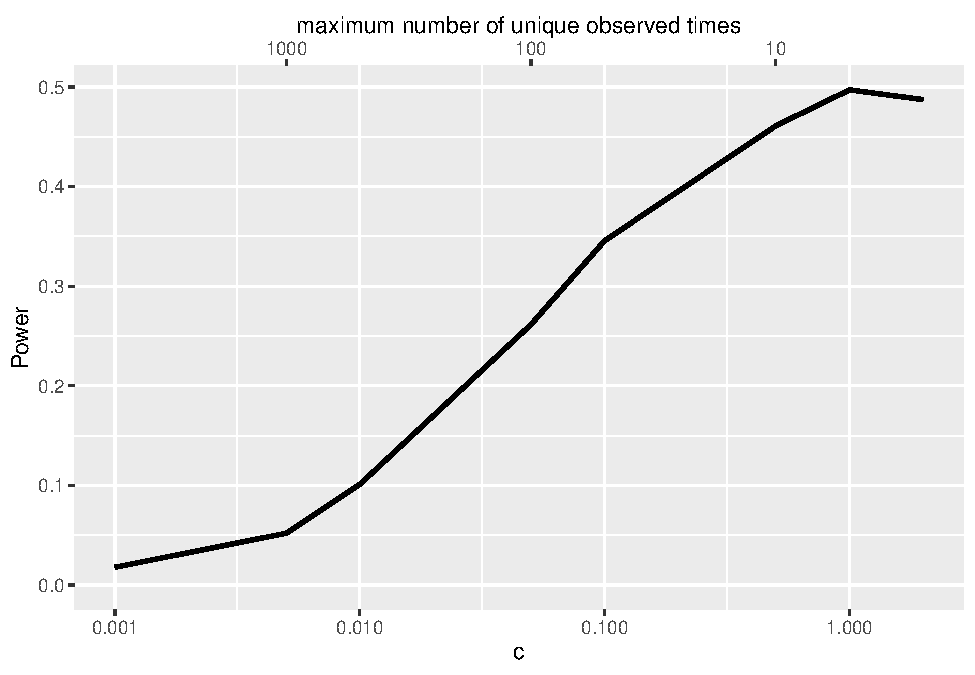
\includegraphics[width=0.6\textwidth]{interval.pdf}
    \caption[Overall power by interval length $c$ and maximum number of unique observed times
    ]{Overall elimination power along the path by interval length $c$ and maximum number of unique observed times.\label{Fig:interval}}
\end{figure}

Note that as $c$ increases and the failure times are grouped into wider intervals, the information they contain decreases and thus the signal-to-noise ratio decreases as well. This would cause the screening power to decrease. As Figure~\ref{Fig:interval} shows, the screening power mostly increases as $c$ increases (and $f$ decreases), as we would expect based on the dimensionality of the dual variable. At some point, however, $c$ becomes too large and the loss in signal dominates, leading to a slight drop in screening power.

\subsubsection{Distribution of Features}

The semiparametric nature of Cox regression not only increases the dimension of $\Theta_\lambda$, but also gives more freedom to $\Theta''$ in Theorem \ref{thm:1}, which controls the shape of the ellipsoid bound for $\Theta_\lambda$. No assumptions are made concerning the underlying distribution of failure times, giving $\Theta''$ the freedom to go to a direction that leads to a ``bad'' shape. The consequences can be seen in the difference between Lemma \ref{lem:3}, where $\Theta''$ is assumed known, and Theorem \ref{thm:2}, which is based on the worst-case value of $\Theta''$. The impact can be interpreted as substituting a weighted variance whose weights $W$ depends on $\Theta''$, with a weighted variance that puts half weight each on the two most extreme points. The ratio between these two terms can be expressed as:
\begin{equation}
    \label{eq:alpharatio}
    \frac{4\sum_{k=1}^fd_k\sum_{i=1}^nW_{ki}\left(X_{ij}-W_k^Tx_j\right)^2}{\sum_{k=1}^fd_k\left(\max_{i:\delta_{ki}=1}X_{ij}-\min_{i:\delta_{ki}=1}X_{ij}\right)^2}
\end{equation}
If this ratio is close to 1, it implies that the extra freedom granted to $\Theta''$ by the lack of parametric assumptions is negligible. This occurs often in practice; for example, when a variable is binary and roughly balanced, the ratio between the two variances will be close to 1. In the following experiment, elements of $X$ are generated from a $\textnormal{Beta}(\alpha,\alpha)$ distribution and we investigate the power of the proposed screening rule as $\alpha$ varies. Note that the distribution of the features is bounded from both ends, with a small value of $\alpha$ putting more weight on the two ends and resembling a balanced binary distribution, while a larger value of $\alpha$ leading to a unimodal bell-shaped distribution and thus, a smaller value of the ratio of weighted variances in \eqref{eq:alpharatio}. In the computation of the numerator in the ratio \eqref{eq:alpharatio}, the weights are assumed to be evenly distributed. Each $x_j$ is also standardized to ensure any differences are not caused by the scale of the feature. 

\begin{figure}[ht]
    \centering
    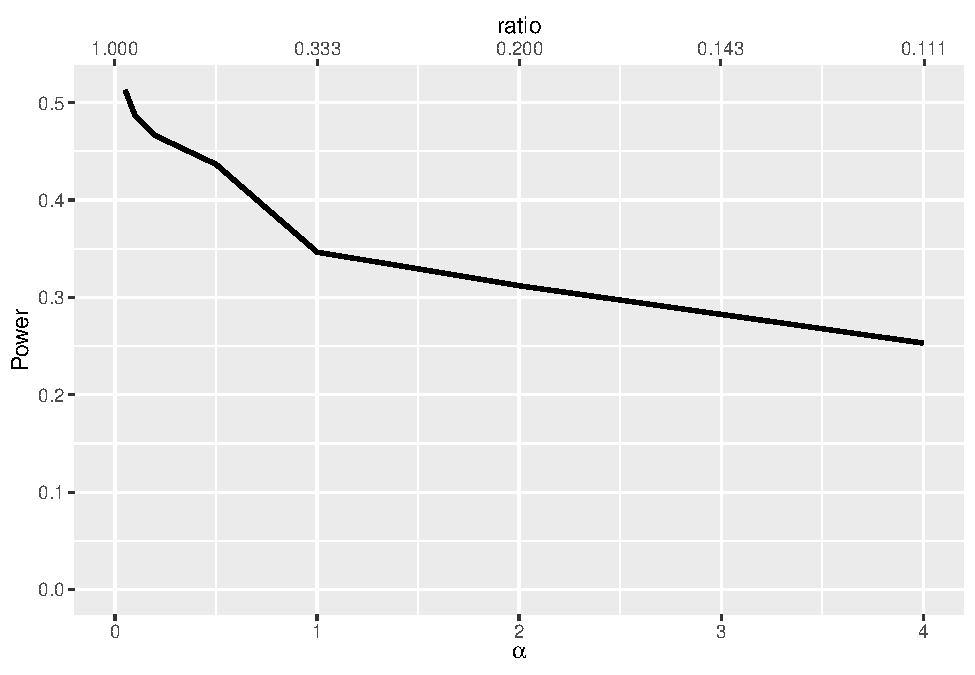
\includegraphics[width=0.6\textwidth]{alpha.pdf}  
    \caption[Overall power by shape $\alpha$ and ratio \eqref{eq:alpharatio}]{Overall elimination power along the path by shape $\alpha$ and ratio \eqref{eq:alpharatio} \label{Fig:alpha}.}
\end{figure}

Figure~\ref{Fig:alpha} summarizes the effect of $\alpha$ on total screening power. As the distribution of $x_j$ puts more weight on the two ends (small $\alpha$), this leads to much better performance, while a distribution of $x_j$ that puts more weight in the center (large $\alpha$) leads to worse performance.

\subsection{Other Common Factors}

In this section, we carry out experiments involving other common factors in the optimization problem to be solved. The results are summarized in Figure~\ref{Fig:coxsim}.

\begin{figure}[ht]
    \centering
    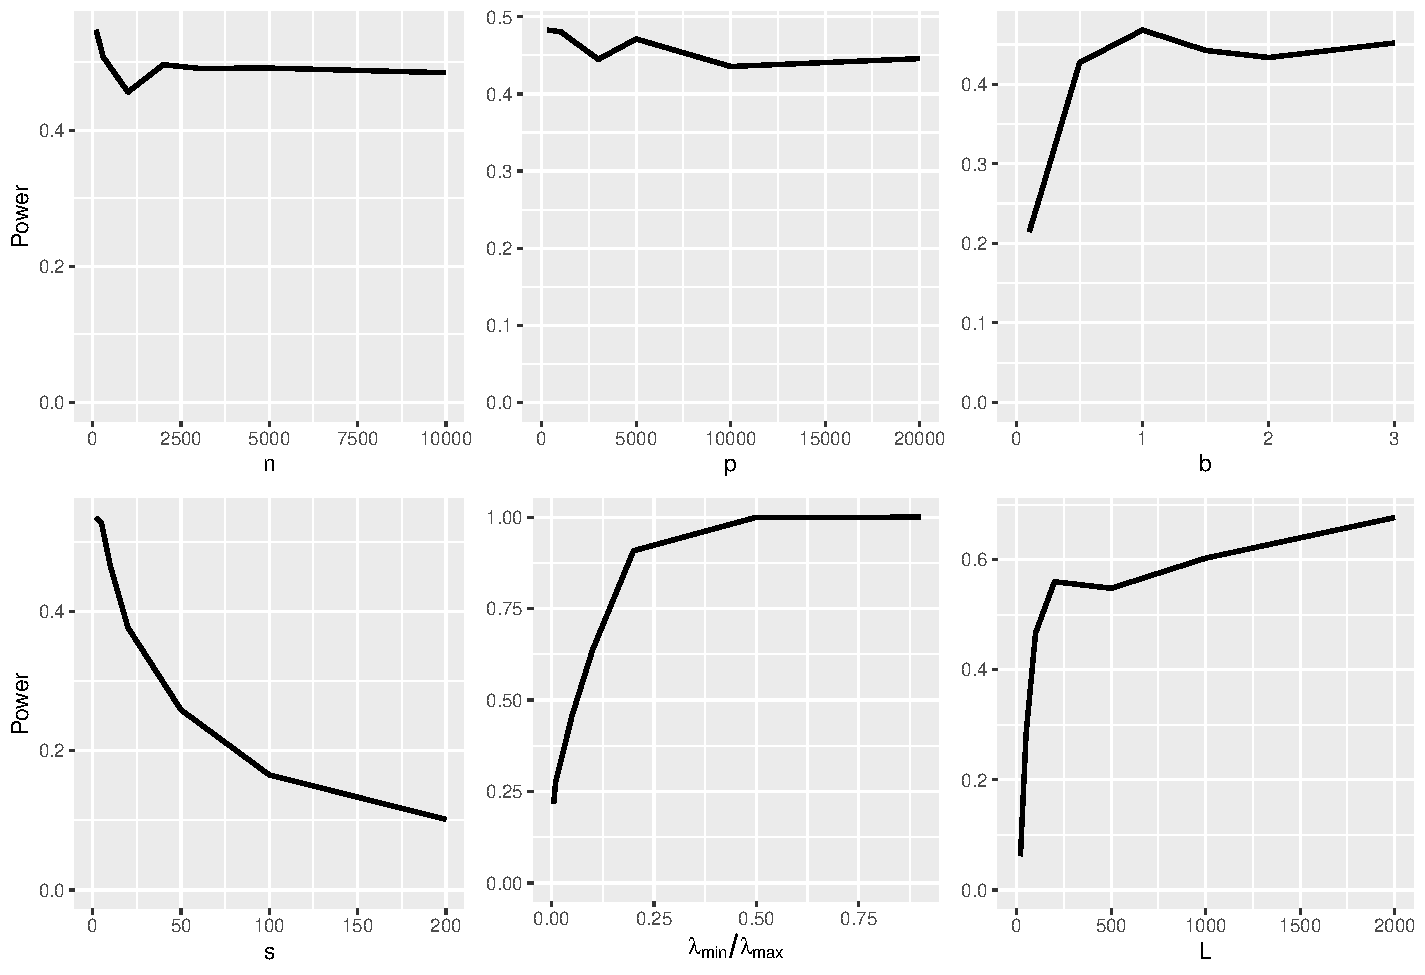
\includegraphics[width=\textwidth]{coxsim.pdf}    
    \caption{Overall elimination power along the path by common factors \label{Fig:coxsim}.}
\end{figure}

In the first row, we vary the sample size $n$, the number of features $p$ and size of coefficients $b$, respectively. None of these factors has a significant impact on the performance, except in the extreme case when $b$ is extremely small and the signal in the data becomes too weak to provide useful information. In the second row, we first vary the number of nonzero coefficients $s$ and see that the screening method performs better when the model is more sparse and a lasso penalty is more appropriate. Second, we vary the ratio $\lambda_{\min}/\lambda_{\max}$. The screening method is more powerful when this ratio is larger, in which case the solution path is more sparse and the $\lambda$ values are more closely spaced. This closer spacing benefits the proposed screening rule, as it means that the previous solution will be closer to the current solution and thus more helpful as a reference. Finally, we vary the number of $\lambda$ values in the solution path and see once again that the screening method is more powerful when $L$ is large and $\lambda$ values more closely spaced.

\section{Application}

In this section, we apply the proposed sequential safe rule to a lasso-penalized Cox regression analysis of data involving lung cancer patients \citep{shedden2008gene}. In the study, the observed time $t_i$ is the number of months since treatment (surgery), with $y_i=1$ representing the death of patient $i$. There are $p=22,304$ features, of which $22,283$ are gene expression levels and the remaining $21$ consisting of various demographic and clinical variables. The sample size is $n=442$ with $236$ failures observed and number of unique failure times $f=204$. The lasso penalized Cox regression problem will be solved along a path of $L=100$ $\lambda$ values equally spaced on log scale between $(0.2\lambda_{\max},\lambda_{\max})$. 

To address the limitations discussed in \ref{sec:lim}, we analyze modified versions of this data in addition to the original, constructed through combination of the following two processes. First, we can bin the observed times into intervals of one-year lengths. This modification reduces the number of unique failure times to $f=14$ and thus, the dimension of the dual variable. Second, we can dichotomize the gene expression features as above/below its sample median. This modification leads to a balanced binary distribution of the features and tightens the ratio in \eqref{eq:alpharatio}. These two modifications represents special cases that also occur in practice. The first modification corresponds to survival data where observed times are recorded in coarse units, while the second corresponds to data where features are recorded in levels of ``high'' and ``low'', instead of raw measurements.

In the following experiment, we compare several different screening methods. For each screening method, the algorithm optimizing the reduced problem after screening is Coordinate Descent \citep{simon2011regularization} with Active Cycling \citep{lee2007efficient}. Active Cycling (AC) is a simple idea similar to screening, where the reduced problem involving only features that are active in the previous solution is first solved and then a KKT condition check is performed to identify other features that must be added to the active set. It can easily be implemented in combination with any screening method and greatly reduces computation cost in most cases, so in this experiment we combine it with all screening methods. We compare the following screening methods: no screening other than AC (AC), basic version of the sequential safe rule that uses only the solution at $\lambda_{\max}$ (Basic), sequential safe rule that uses previous solution (Sequential), sequential strong rule (SSR) and adaptive screening built on the sequential safe rule (Adaptive).

Table \ref{Tab:realcox} summarizes the total computation cost in seconds across all combinations of screening method and dataset. In the dataset with coarse observed times and binary features (Both Modified), the sequential safe screening provides significant speedup over AC, and is close in performance to the sequential strong rule. Moreover, an adaptive screening approach using the proposed safe rule outperforms all other screening methods in this case. The adaptive screening method is also robust and is close to fastest under all cases.

\begin{table}[H]
\centering
\begin{tabular}{lllll}
\toprule
Screening  & Original Data & Modified Times & Modified Features & Both Modified \\
\midrule
AC & 2.386 (0.003) & 1.889 (0.005) & 2.342 (0.004) & 1.869 (0.004) \\
Basic & 2.463 (0.003) & 1.919 (0.003) & 2.288 (0.004) & 1.906 (0.004) \\
Sequential & 2.911 (0.003) & 2.262 (0.004) & 2.447 (0.006) & 1.306 (0.005) \\
SSR & \textbf{1.254 (0.003)} & \textbf{1.055 (0.004)} & \textbf{1.225 (0.003)} & 1.030 (0.003) \\
Adaptive & 1.302 (0.004) & 1.078 (0.002) & 1.255 (0.003) & \textbf{0.769 (0.003)} \\
\bottomrule
\end{tabular}
\caption{Average computing time in seconds (standard error) for lasso penalized Cox regression on different modified data sets.}
\label{Tab:realcox}
\end{table}

Figure~\ref{Fig:shedden} shows the number of features eliminated by the proposed sequential safe rule at each $\lambda$ value for each dataset, and shows the considerable impact of the modifications on the power of the screening rule. Although the rule is almost entirely ineffective on the original data, with a smaller number of unique failure times and a binary distribution of features, the the rule becomes much more powerful at eliminating features.

\begin{figure}[ht]
    \centering
    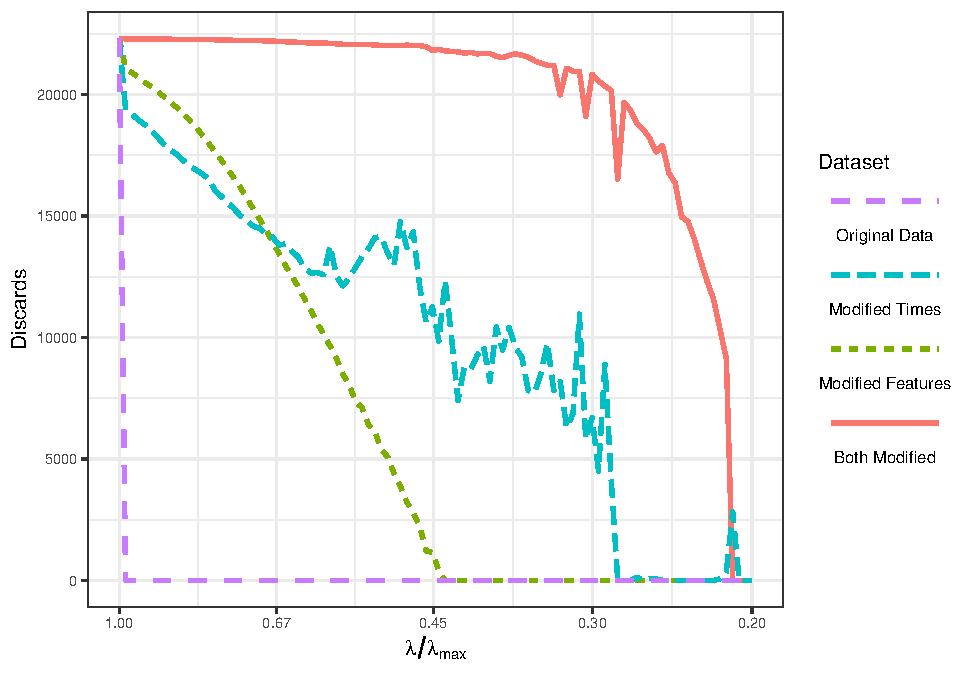
\includegraphics[width=0.7\textwidth]{shedden.pdf}    
    \caption{Number of eliminated features along the path for lasso penalized Cox regression on different modified data sets\label{Fig:shedden}.}
\end{figure}